\label{sec:BundleWidth}
Based on the decussation and targeting phenotype in the EphB1\textsuperscript{-/-} mutant and the increasing evidence that Ephs and ephrins are involved in fasciculation and axon sorting, I chose to further pursue questions of pre-target axon organization in the EphB1\textsuperscript{-/-} mutant optic tract.
This exploration is two-fold.
First, I used the EphB1\textsuperscript{-/-} mutant as a model to link three steps in retinogeniculate circuit development: midline choice, tract organization, and targeting.
Understanding how axons are organized in the tract in between the midline and the target can help clarify the role of axon tract organization in the development of the overall circuit.
The EphB1\textsuperscript{-/-} mutant is particularly useful for this purpose, because EphB1\textsuperscript{-/-} axons aberrantly cross at the midline but target grossly normally, albeit with incorrect laterality.
That is, there is an incorrect midline choice but broadly correct targeting.
Therefore, asking where the aberrantly crossed axons are located in the tract (with the remaining ipsi axons or with the normal contra axons), can begin to address the relationship between midline choice, tract order, and targeting.
\begin{figure}[hbtp]
    \begin{center}
        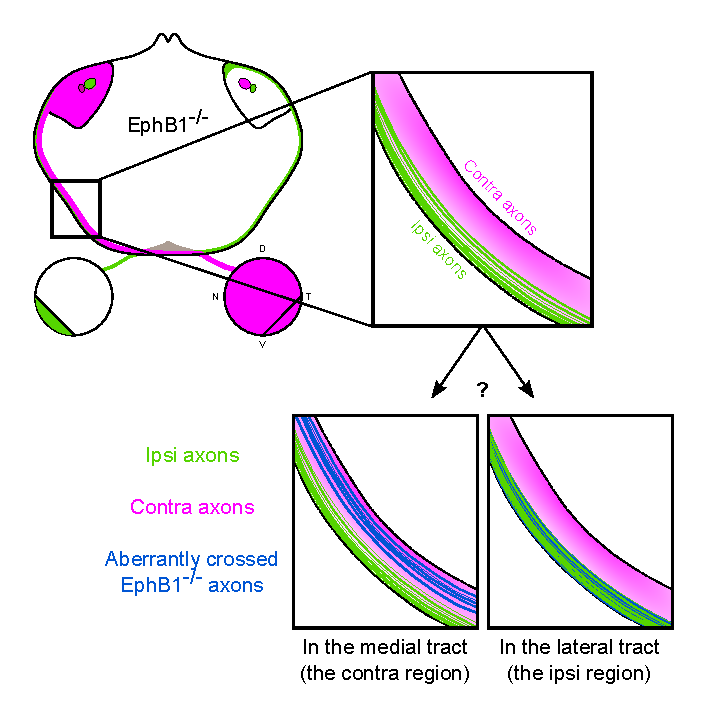
\includegraphics{Figures/EphB1_Sert_schematic.pdf}
        \caption[Schematic of possible position of aberrantly decussated axons in the EphB1\textsuperscript{-/-} optic tract.]
        {Schematic of possible position of aberrantly decussated axons in the EphB1\textsuperscript{-/-} optic tract.
        The EphB1\textsuperscript{-/-} retinogeniculate pathway is illustrated at top.
        Bottom panels show two possible positions of aberrantly crossing EphB1\textsuperscript{-/-} axons (blue) in the optic tract, relative to the normal ipsi (green) and contra (pink) components.
        }
        \label{EphB1Sertschematic}
    \end{center}
\end{figure}

If axon organization in the optic tract is unimportant for eventual targeting decisions, then the aberrantly crossing axons in the EphB1\textsuperscript{-/-} tract would likely commingle with the normal contra RGC axon population.
In this case, local cues in the dLGN to which the aberrantly crossing axons remain sensitive could be sufficient for corralling them to the ipsi-recipient zone of the dLGN.
If, on the other hand, aberrantly crossing EphB1\textsuperscript{-/-} axons associate with the remaining ipsi RGC axons of the contralateral tract, then a model in which pre-target axon organization is important for targeting would be favored.
The latter finding would provide indirect evidence that bundling partners in the tract are important for guiding axons to their appropriate target region.
These two possibilities of axon organization in the EphB1\textsuperscript{-/-} optic tract are illustrated in Figure~\ref{EphB1Sertschematic}.

The second aspect of my exploration of the EphB1\textsuperscript{-/-} mutant relates more specifically to ipsi RGC axon fasciculation.
Findings discussed in Section~\ref{sec:EphFascic} indicate that Ephs and ephrins are involved in surround repulsion mediated fasciculation and in direct inter-axonal interactions important for sorting cohorts of axons in their tracts.
Because EphB1 is expressed by ipsi RGCs, it could be involved in ipsi-specific fasciculation behavior, which I described in vitro in the previous chapter.

Thus, in this chapter, I will present my findings addressing three questions.
First, how does loss of EphB1 and reduction of the ipsi component affect the overall eye-specific organization of the optic tract?
Second, where are aberrantly crossing EphB\textsuperscript{-/-} axons located in the optic tract relative to the normal ipsi and contra cohorts of RGC axons?
Third, does loss of EphB1 affect ipsi neurite fasciculation in vitro?